\documentclass[1p]{elsarticle_modified}
%\bibliographystyle{elsarticle-num}

%\usepackage[colorlinks]{hyperref}
%\usepackage{abbrmath_seonhwa} %\Abb, \Ascr, \Acal ,\Abf, \Afrak
\usepackage{amsfonts}
\usepackage{amssymb}
\usepackage{amsmath}
\usepackage{amsthm}
\usepackage{scalefnt}
\usepackage{amsbsy}
\usepackage{kotex}
\usepackage{caption}
\usepackage{subfig}
\usepackage{color}
\usepackage{graphicx}
\usepackage{xcolor} %% white, black, red, green, blue, cyan, magenta, yellow
\usepackage{float}
\usepackage{setspace}
\usepackage{hyperref}

\usepackage{tikz}
\usetikzlibrary{arrows}

\usepackage{multirow}
\usepackage{array} % fixed length table
\usepackage{hhline}

%%%%%%%%%%%%%%%%%%%%%
\makeatletter
\renewcommand*\env@matrix[1][\arraystretch]{%
	\edef\arraystretch{#1}%
	\hskip -\arraycolsep
	\let\@ifnextchar\new@ifnextchar
	\array{*\c@MaxMatrixCols c}}
\makeatother %https://tex.stackexchange.com/questions/14071/how-can-i-increase-the-line-spacing-in-a-matrix
%%%%%%%%%%%%%%%

\usepackage[normalem]{ulem}

\newcommand{\msout}[1]{\ifmmode\text{\sout{\ensuremath{#1}}}\else\sout{#1}\fi}
%SOURCE: \msout is \stkout macro in https://tex.stackexchange.com/questions/20609/strikeout-in-math-mode

\newcommand{\cancel}[1]{
	\ifmmode
	{\color{red}\msout{#1}}
	\else
	{\color{red}\sout{#1}}
	\fi
}

\newcommand{\add}[1]{
	{\color{blue}\uwave{#1}}
}

\newcommand{\replace}[2]{
	\ifmmode
	{\color{red}\msout{#1}}{\color{blue}\uwave{#2}}
	\else
	{\color{red}\sout{#1}}{\color{blue}\uwave{#2}}
	\fi
}

\newcommand{\Sol}{\mathcal{S}} %segment
\newcommand{\D}{D} %diagram
\newcommand{\A}{\mathcal{A}} %arc


%%%%%%%%%%%%%%%%%%%%%%%%%%%%%5 test

\def\sl{\operatorname{\textup{SL}}(2,\Cbb)}
\def\psl{\operatorname{\textup{PSL}}(2,\Cbb)}
\def\quan{\mkern 1mu \triangleright \mkern 1mu}

\theoremstyle{definition}
\newtheorem{thm}{Theorem}[section]
\newtheorem{prop}[thm]{Proposition}
\newtheorem{lem}[thm]{Lemma}
\newtheorem{ques}[thm]{Question}
\newtheorem{cor}[thm]{Corollary}
\newtheorem{defn}[thm]{Definition}
\newtheorem{exam}[thm]{Example}
\newtheorem{rmk}[thm]{Remark}
\newtheorem{alg}[thm]{Algorithm}

\newcommand{\I}{\sqrt{-1}}
\begin{document}

%\begin{frontmatter}
%
%\title{Boundary parabolic representations of knots up to 8 crossings}
%
%%% Group authors per affiliation:
%\author{Yunhi Cho} 
%\address{Department of Mathematics, University of Seoul, Seoul, Korea}
%\ead{yhcho@uos.ac.kr}
%
%
%\author{Seonhwa Kim} %\fnref{s_kim}}
%\address{Center for Geometry and Physics, Institute for Basic Science, Pohang, 37673, Korea}
%\ead{ryeona17@ibs.re.kr}
%
%\author{Hyuk Kim}
%\address{Department of Mathematical Sciences, Seoul National University, Seoul 08826, Korea}
%\ead{hyukkim@snu.ac.kr}
%
%\author{Seokbeom Yoon}
%\address{Department of Mathematical Sciences, Seoul National University, Seoul, 08826,  Korea}
%\ead{sbyoon15@snu.ac.kr}
%
%\begin{abstract}
%We find all boundary parabolic representation of knots up to 8 crossings.
%
%\end{abstract}
%\begin{keyword}
%    \MSC[2010] 57M25 
%\end{keyword}
%
%\end{frontmatter}

%\linenumbers
%\tableofcontents
%
\newcommand\colored[1]{\textcolor{white}{\rule[-0.35ex]{0.8em}{1.4ex}}\kern-0.8em\color{red} #1}%
%\newcommand\colored[1]{\textcolor{white}{ #1}\kern-2.17ex	\textcolor{white}{ #1}\kern-1.81ex	\textcolor{white}{ #1}\kern-2.15ex\color{red}#1	}

{\Large $\underline{12a_{0240}~(K12a_{0240})}$}

\setlength{\tabcolsep}{10pt}
\renewcommand{\arraystretch}{1.6}
\vspace{1cm}\begin{tabular}{m{100pt}>{\centering\arraybackslash}m{274pt}}
\multirow{5}{120pt}{
	\centering
	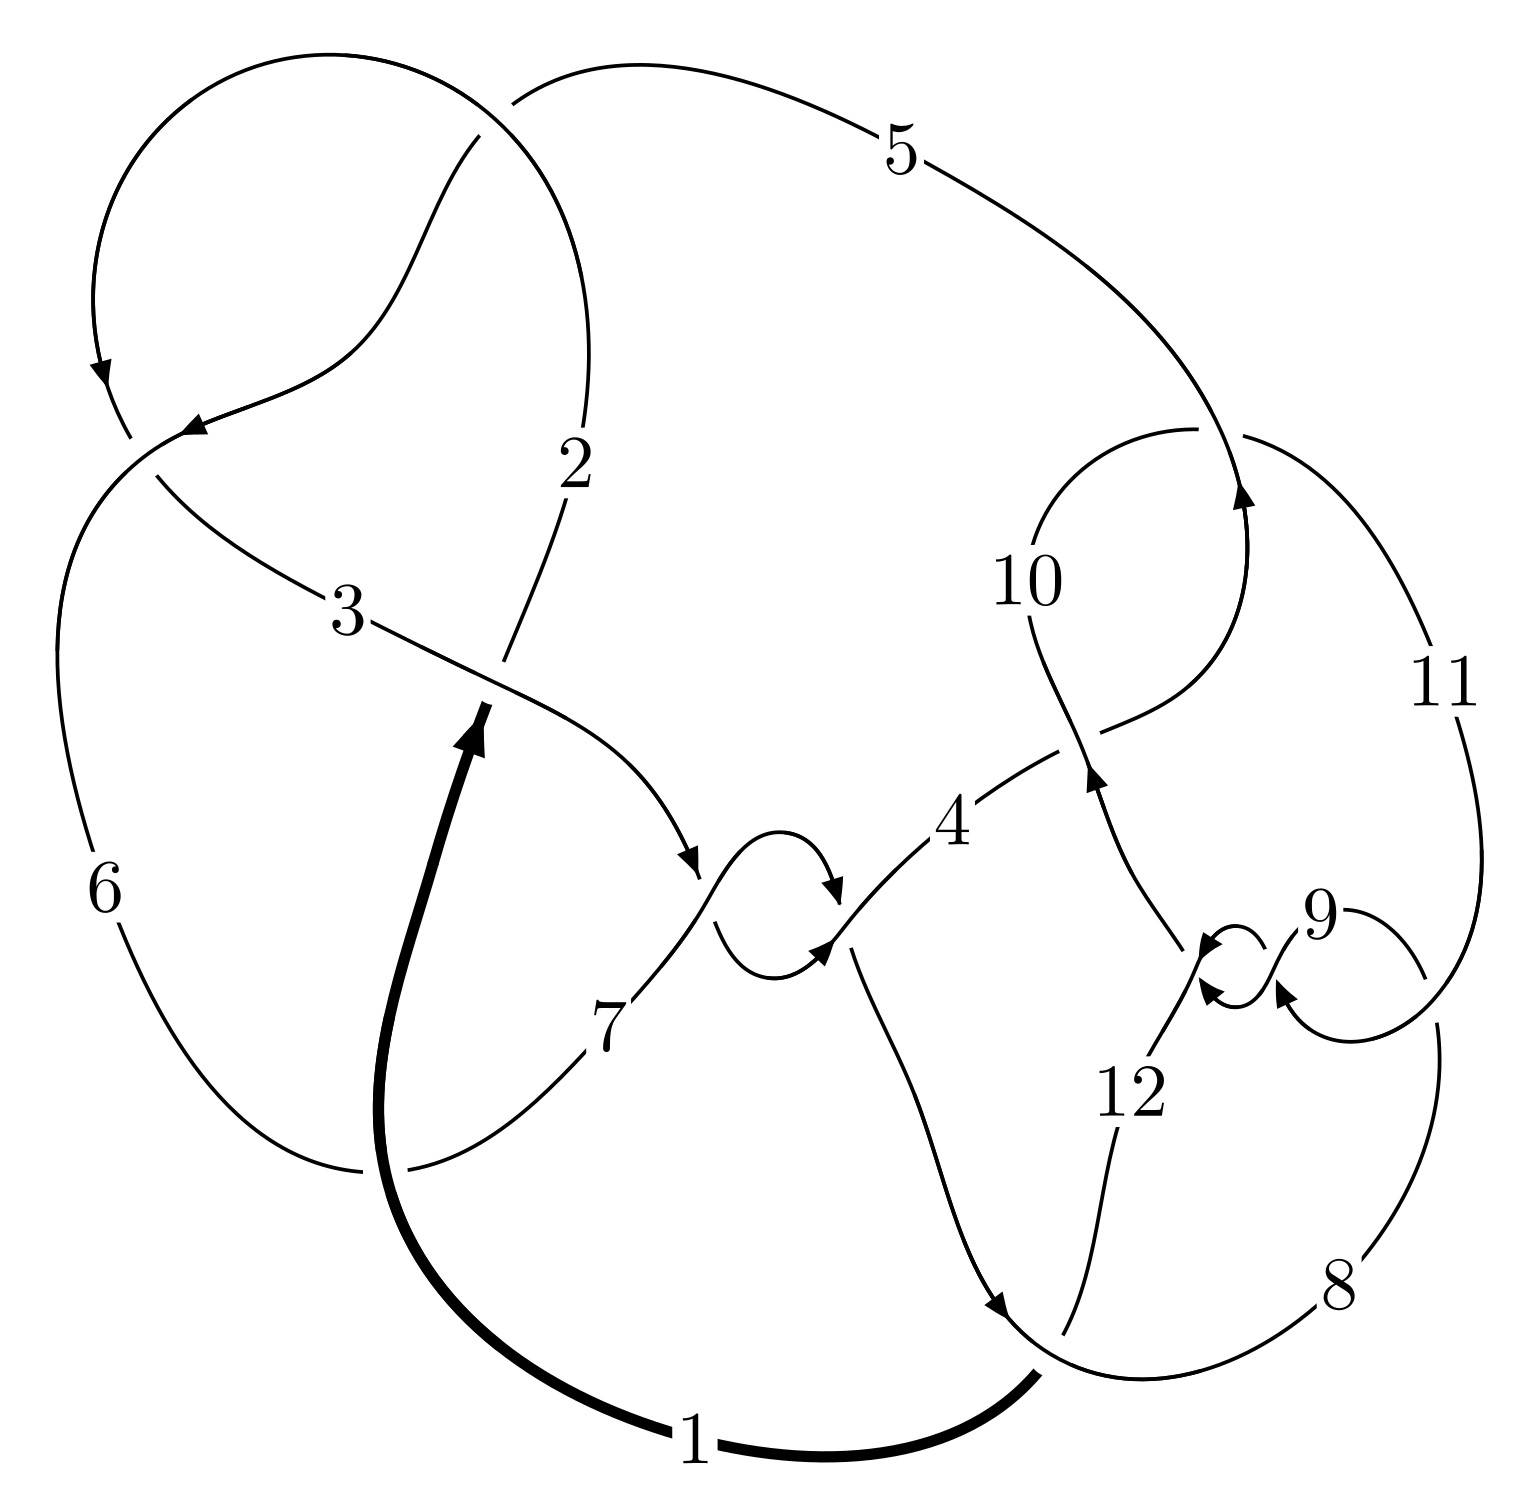
\includegraphics[width=112pt]{../../../GIT/diagram.site/Diagrams/png/1041_12a_0240.png}\\
\ \ \ A knot diagram\footnotemark}&
\allowdisplaybreaks
\textbf{Linearized knot diagam} \\
\cline{2-2}
 &
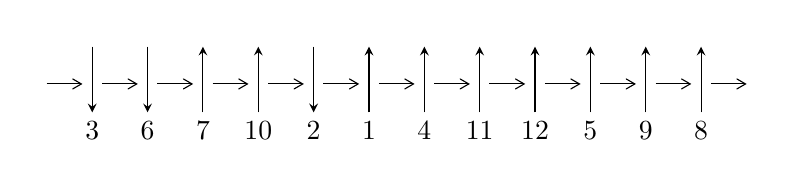
\begin{tikzpicture}[x=20pt, y=17pt]
	% nodes
	\node (C0) at (0, 0) {};
	\node (C1) at (1, 0) {};
	\node (C1U) at (1, +1) {};
	\node (C1D) at (1, -1) {3};

	\node (C2) at (2, 0) {};
	\node (C2U) at (2, +1) {};
	\node (C2D) at (2, -1) {6};

	\node (C3) at (3, 0) {};
	\node (C3U) at (3, +1) {};
	\node (C3D) at (3, -1) {7};

	\node (C4) at (4, 0) {};
	\node (C4U) at (4, +1) {};
	\node (C4D) at (4, -1) {10};

	\node (C5) at (5, 0) {};
	\node (C5U) at (5, +1) {};
	\node (C5D) at (5, -1) {2};

	\node (C6) at (6, 0) {};
	\node (C6U) at (6, +1) {};
	\node (C6D) at (6, -1) {1};

	\node (C7) at (7, 0) {};
	\node (C7U) at (7, +1) {};
	\node (C7D) at (7, -1) {4};

	\node (C8) at (8, 0) {};
	\node (C8U) at (8, +1) {};
	\node (C8D) at (8, -1) {11};

	\node (C9) at (9, 0) {};
	\node (C9U) at (9, +1) {};
	\node (C9D) at (9, -1) {12};

	\node (C10) at (10, 0) {};
	\node (C10U) at (10, +1) {};
	\node (C10D) at (10, -1) {5};

	\node (C11) at (11, 0) {};
	\node (C11U) at (11, +1) {};
	\node (C11D) at (11, -1) {9};

	\node (C12) at (12, 0) {};
	\node (C12U) at (12, +1) {};
	\node (C12D) at (12, -1) {8};
	\node (C13) at (13, 0) {};

	% arrows
	\draw[->,>={angle 60}]
	(C0) edge (C1) (C1) edge (C2) (C2) edge (C3) (C3) edge (C4) (C4) edge (C5) (C5) edge (C6) (C6) edge (C7) (C7) edge (C8) (C8) edge (C9) (C9) edge (C10) (C10) edge (C11) (C11) edge (C12) (C12) edge (C13) ;	\draw[->,>=stealth]
	(C1U) edge (C1D) (C2U) edge (C2D) (C3D) edge (C3U) (C4D) edge (C4U) (C5U) edge (C5D) (C6D) edge (C6U) (C7D) edge (C7U) (C8D) edge (C8U) (C9D) edge (C9U) (C10D) edge (C10U) (C11D) edge (C11U) (C12D) edge (C12U) ;
	\end{tikzpicture} \\
\hhline{~~} \\& 
\textbf{Solving Sequence} \\ \cline{2-2} 
 &
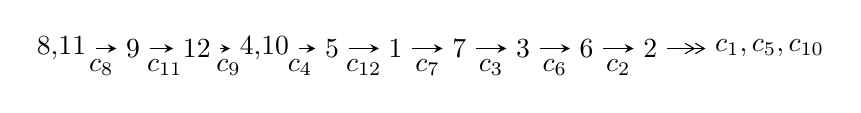
\begin{tikzpicture}[x=23pt, y=7pt]
	% node
	\node (A0) at (-1/8, 0) {8,11};
	\node (A1) at (1, 0) {9};
	\node (A2) at (2, 0) {12};
	\node (A3) at (49/16, 0) {4,10};
	\node (A4) at (33/8, 0) {5};
	\node (A5) at (41/8, 0) {1};
	\node (A6) at (49/8, 0) {7};
	\node (A7) at (57/8, 0) {3};
	\node (A8) at (65/8, 0) {6};
	\node (A9) at (73/8, 0) {2};
	\node (C1) at (1/2, -1) {$c_{8}$};
	\node (C2) at (3/2, -1) {$c_{11}$};
	\node (C3) at (5/2, -1) {$c_{9}$};
	\node (C4) at (29/8, -1) {$c_{4}$};
	\node (C5) at (37/8, -1) {$c_{12}$};
	\node (C6) at (45/8, -1) {$c_{7}$};
	\node (C7) at (53/8, -1) {$c_{3}$};
	\node (C8) at (61/8, -1) {$c_{6}$};
	\node (C9) at (69/8, -1) {$c_{2}$};
	\node (A10) at (11, 0) {$c_{1},c_{5},c_{10}$};

	% edge
	\draw[->,>=stealth]	
	(A0) edge (A1) (A1) edge (A2) (A2) edge (A3) (A3) edge (A4) (A4) edge (A5) (A5) edge (A6) (A6) edge (A7) (A7) edge (A8) (A8) edge (A9) ;
	\draw[->>,>={angle 60}]	
	(A9) edge (A10);
\end{tikzpicture} \\ 

\end{tabular} \\

\footnotetext{
The image of knot diagram is generated by the software ``\textbf{Draw programme}" developed by Andrew Bartholomew(\url{http://www.layer8.co.uk/maths/draw/index.htm\#Running-draw}), where we modified some parts for our purpose(\url{https://github.com/CATsTAILs/LinksPainter}).
}\phantom \\ \newline 
\centering \textbf{Ideals for irreducible components\footnotemark of $X_{\text{par}}$} 
 
\begin{align*}
I^u_{1}&=\langle 
43 u^{91}-1146 u^{90}+\cdots+32 b+579,\;141 u^{91}-878 u^{90}+\cdots+4 a+144,\;u^{92}-7 u^{91}+\cdots+3 u-1\rangle \\
I^u_{2}&=\langle 
b^6+b^5- b^4-2 b^3+b+1,\;a,\;u+1\rangle \\
\\
\end{align*}
\raggedright * 2 irreducible components of $\dim_{\mathbb{C}}=0$, with total 98 representations.\\
\footnotetext{All coefficients of polynomials are rational numbers. But the coefficients are sometimes approximated in decimal forms when there is not enough margin.}
\newpage
\renewcommand{\arraystretch}{1}
\centering \section*{I. $I^u_{1}= \langle 43 u^{91}-1146 u^{90}+\cdots+32 b+579,\;141 u^{91}-878 u^{90}+\cdots+4 a+144,\;u^{92}-7 u^{91}+\cdots+3 u-1 \rangle$}
\flushleft \textbf{(i) Arc colorings}\\
\begin{tabular}{m{7pt} m{180pt} m{7pt} m{180pt} }
\flushright $a_{8}=$&$\begin{pmatrix}1\\0\end{pmatrix}$ \\
\flushright $a_{11}=$&$\begin{pmatrix}0\\u\end{pmatrix}$ \\
\flushright $a_{9}=$&$\begin{pmatrix}1\\- u^2\end{pmatrix}$ \\
\flushright $a_{12}=$&$\begin{pmatrix}u\\- u^3+u\end{pmatrix}$ \\
\flushright $a_{4}=$&$\begin{pmatrix}-\frac{141}{4} u^{91}+\frac{439}{2} u^{90}+\cdots+80 u-36\\-1.34375 u^{91}+35.8125 u^{90}+\cdots+26.1875 u-18.0938\end{pmatrix}$ \\
\flushright $a_{10}=$&$\begin{pmatrix}- u^2+1\\u^4-2 u^2\end{pmatrix}$ \\
\flushright $a_{5}=$&$\begin{pmatrix}\frac{259}{2} u^{91}-723 u^{90}+\cdots-\frac{407}{2} u+\frac{359}{4}\\84.1563 u^{91}-414.438 u^{90}+\cdots-88.5625 u+26.4063\end{pmatrix}$ \\
\flushright $a_{1}=$&$\begin{pmatrix}- u^3+2 u\\- u^3+u\end{pmatrix}$ \\
\flushright $a_{7}=$&$\begin{pmatrix}- u^9+4 u^7+2 u^6-5 u^5-6 u^4+4 u^2+3 u+2\\0.0312500 u^{91}-0.187500 u^{90}+\cdots-1.06250 u+0.0312500\end{pmatrix}$ \\
\flushright $a_{3}=$&$\begin{pmatrix}73.0313 u^{91}-436.188 u^{90}+\cdots-135.313 u+68.5313\\367.031 u^{91}-2093.25 u^{90}+\cdots-628.625 u+279.844\end{pmatrix}$ \\
\flushright $a_{6}=$&$\begin{pmatrix}-0.0312500 u^{91}+0.187500 u^{90}+\cdots+3.06250 u+1.96875\\0.0312500 u^{91}-0.187500 u^{90}+\cdots-1.06250 u+0.0312500\end{pmatrix}$ \\
\flushright $a_{2}=$&$\begin{pmatrix}2.68750 u^{91}-15.9375 u^{90}+\cdots+4.81250 u+3.50000\\15.4688 u^{91}-91.0625 u^{90}+\cdots-29.1875 u+13.8438\end{pmatrix}$\\&\end{tabular}
\flushleft \textbf{(ii) Obstruction class $= -1$}\\~\\
\flushleft \textbf{(iii) Cusp Shapes $= -\frac{3517}{8} u^{91}+\frac{39449}{16} u^{90}+\cdots+\frac{11229}{16} u-\frac{4837}{16}$}\\~\\
\newpage\renewcommand{\arraystretch}{1}
\flushleft \textbf{(iv) u-Polynomials at the component}\newline \\
\begin{tabular}{m{50pt}|m{274pt}}
Crossings & \hspace{64pt}u-Polynomials at each crossing \\
\hline $$\begin{aligned}c_{1}\end{aligned}$$&$\begin{aligned}
&u^{92}+42 u^{91}+\cdots+6 u+1
\end{aligned}$\\
\hline $$\begin{aligned}c_{2},c_{5}\end{aligned}$$&$\begin{aligned}
&u^{92}+2 u^{91}+\cdots-2 u+1
\end{aligned}$\\
\hline $$\begin{aligned}c_{3},c_{7}\end{aligned}$$&$\begin{aligned}
&u^{92}-2 u^{91}+\cdots+110 u+25
\end{aligned}$\\
\hline $$\begin{aligned}c_{4},c_{10}\end{aligned}$$&$\begin{aligned}
&u^{92}- u^{91}+\cdots+128 u-64
\end{aligned}$\\
\hline $$\begin{aligned}c_{6}\end{aligned}$$&$\begin{aligned}
&u^{92}+6 u^{91}+\cdots-18 u-5
\end{aligned}$\\
\hline $$\begin{aligned}c_{8},c_{9},c_{11}\end{aligned}$$&$\begin{aligned}
&u^{92}+7 u^{91}+\cdots-3 u-1
\end{aligned}$\\
\hline $$\begin{aligned}c_{12}\end{aligned}$$&$\begin{aligned}
&u^{92}-39 u^{91}+\cdots-45056 u+4096
\end{aligned}$\\
\hline
\end{tabular}\\~\\
\newpage\renewcommand{\arraystretch}{1}
\flushleft \textbf{(v) Riley Polynomials at the component}\newline \\
\begin{tabular}{m{50pt}|m{274pt}}
Crossings & \hspace{64pt}Riley Polynomials at each crossing \\
\hline $$\begin{aligned}c_{1}\end{aligned}$$&$\begin{aligned}
&y^{92}+18 y^{91}+\cdots-50 y+1
\end{aligned}$\\
\hline $$\begin{aligned}c_{2},c_{5}\end{aligned}$$&$\begin{aligned}
&y^{92}-42 y^{91}+\cdots-6 y+1
\end{aligned}$\\
\hline $$\begin{aligned}c_{3},c_{7}\end{aligned}$$&$\begin{aligned}
&y^{92}-66 y^{91}+\cdots+23850 y+625
\end{aligned}$\\
\hline $$\begin{aligned}c_{4},c_{10}\end{aligned}$$&$\begin{aligned}
&y^{92}-39 y^{91}+\cdots-45056 y+4096
\end{aligned}$\\
\hline $$\begin{aligned}c_{6}\end{aligned}$$&$\begin{aligned}
&y^{92}+6 y^{91}+\cdots+1086 y+25
\end{aligned}$\\
\hline $$\begin{aligned}c_{8},c_{9},c_{11}\end{aligned}$$&$\begin{aligned}
&y^{92}-81 y^{91}+\cdots+y+1
\end{aligned}$\\
\hline $$\begin{aligned}c_{12}\end{aligned}$$&$\begin{aligned}
&y^{92}+17 y^{91}+\cdots-201326592 y+16777216
\end{aligned}$\\
\hline
\end{tabular}\\~\\
\newpage\flushleft \textbf{(vi) Complex Volumes and Cusp Shapes}
$$\begin{array}{c|c|c}  
\text{Solutions to }I^u_{1}& \I (\text{vol} + \sqrt{-1}CS) & \text{Cusp shape}\\
 \hline 
\begin{aligned}
u &= -0.855893 + 0.527606 I \\
a &= \phantom{-}0.393530 - 0.308819 I \\
b &= \phantom{-}1.238450 - 0.035861 I\end{aligned}
 & \phantom{-}5.58340 - 0.40937 I & \phantom{-0.000000 } 0 \\ \hline\begin{aligned}
u &= -0.855893 - 0.527606 I \\
a &= \phantom{-}0.393530 + 0.308819 I \\
b &= \phantom{-}1.238450 + 0.035861 I\end{aligned}
 & \phantom{-}5.58340 + 0.40937 I & \phantom{-0.000000 } 0 \\ \hline\begin{aligned}
u &= -0.823622 + 0.543416 I \\
a &= -0.299409 + 0.297378 I \\
b &= -1.200290 + 0.200271 I\end{aligned}
 & \phantom{-}3.94188 - 5.47839 I & \phantom{-0.000000 } 0 \\ \hline\begin{aligned}
u &= -0.823622 - 0.543416 I \\
a &= -0.299409 - 0.297378 I \\
b &= -1.200290 - 0.200271 I\end{aligned}
 & \phantom{-}3.94188 + 5.47839 I & \phantom{-0.000000 } 0 \\ \hline\begin{aligned}
u &= -0.934785 + 0.428419 I \\
a &= -0.640037 + 0.141332 I \\
b &= -0.946030 - 0.426464 I\end{aligned}
 & \phantom{-}0.419646 + 0.395087 I & \phantom{-0.000000 } 0 \\ \hline\begin{aligned}
u &= -0.934785 - 0.428419 I \\
a &= -0.640037 - 0.141332 I \\
b &= -0.946030 + 0.426464 I\end{aligned}
 & \phantom{-}0.419646 - 0.395087 I & \phantom{-0.000000 } 0 \\ \hline\begin{aligned}
u &= -0.926309 + 0.516475 I \\
a &= \phantom{-}0.581393 - 0.353795 I \\
b &= \phantom{-}1.344830 + 0.308771 I\end{aligned}
 & \phantom{-}5.25124 + 2.21296 I & \phantom{-0.000000 } 0 \\ \hline\begin{aligned}
u &= -0.926309 - 0.516475 I \\
a &= \phantom{-}0.581393 + 0.353795 I \\
b &= \phantom{-}1.344830 - 0.308771 I\end{aligned}
 & \phantom{-}5.25124 - 2.21296 I & \phantom{-0.000000 } 0 \\ \hline\begin{aligned}
u &= -0.951668 + 0.520377 I \\
a &= -0.650526 + 0.382532 I \\
b &= -1.40538 - 0.44067 I\end{aligned}
 & \phantom{-}3.32536 + 7.33336 I & \phantom{-0.000000 } 0 \\ \hline\begin{aligned}
u &= -0.951668 - 0.520377 I \\
a &= -0.650526 - 0.382532 I \\
b &= -1.40538 + 0.44067 I\end{aligned}
 & \phantom{-}3.32536 - 7.33336 I & \phantom{-0.000000 } 0\\
 \hline 
 \end{array}$$\newpage$$\begin{array}{c|c|c}  
\text{Solutions to }I^u_{1}& \I (\text{vol} + \sqrt{-1}CS) & \text{Cusp shape}\\
 \hline 
\begin{aligned}
u &= -0.257095 + 0.850924 I \\
a &= -1.05101 + 1.49174 I \\
b &= -1.50653 + 0.51583 I\end{aligned}
 & \phantom{-}1.19521 - 12.17710 I & \phantom{-0.000000 } 0 \\ \hline\begin{aligned}
u &= -0.257095 - 0.850924 I \\
a &= -1.05101 - 1.49174 I \\
b &= -1.50653 - 0.51583 I\end{aligned}
 & \phantom{-}1.19521 + 12.17710 I & \phantom{-0.000000 } 0 \\ \hline\begin{aligned}
u &= -0.266178 + 0.838902 I \\
a &= \phantom{-}1.01110 - 1.43448 I \\
b &= \phantom{-}1.41908 - 0.41643 I\end{aligned}
 & \phantom{-}3.21993 - 7.00055 I & \phantom{-0.000000 } 0 \\ \hline\begin{aligned}
u &= -0.266178 - 0.838902 I \\
a &= \phantom{-}1.01110 + 1.43448 I \\
b &= \phantom{-}1.41908 + 0.41643 I\end{aligned}
 & \phantom{-}3.21993 + 7.00055 I & \phantom{-0.000000 } 0 \\ \hline\begin{aligned}
u &= -0.298969 + 0.807596 I \\
a &= \phantom{-}0.91610 - 1.25406 I \\
b &= \phantom{-}1.201580 - 0.120872 I\end{aligned}
 & \phantom{-}3.86636 - 4.28759 I & \phantom{-0.000000 } 0 \\ \hline\begin{aligned}
u &= -0.298969 - 0.807596 I \\
a &= \phantom{-}0.91610 + 1.25406 I \\
b &= \phantom{-}1.201580 + 0.120872 I\end{aligned}
 & \phantom{-}3.86636 + 4.28759 I & \phantom{-0.000000 } 0 \\ \hline\begin{aligned}
u &= -0.320326 + 0.790880 I \\
a &= -0.86648 + 1.14685 I \\
b &= -1.082220 - 0.039888 I\end{aligned}
 & \phantom{-}2.40332 + 0.79509 I & \phantom{-0.000000 } 0 \\ \hline\begin{aligned}
u &= -0.320326 - 0.790880 I \\
a &= -0.86648 - 1.14685 I \\
b &= -1.082220 + 0.039888 I\end{aligned}
 & \phantom{-}2.40332 - 0.79509 I & \phantom{-0.000000 } 0 \\ \hline\begin{aligned}
u &= -0.238388 + 0.811798 I \\
a &= -0.85620 + 1.51375 I \\
b &= -1.149650 + 0.585085 I\end{aligned}
 & -1.74435 - 4.87706 I & \phantom{-0.000000 } 0 \\ \hline\begin{aligned}
u &= -0.238388 - 0.811798 I \\
a &= -0.85620 - 1.51375 I \\
b &= -1.149650 - 0.585085 I\end{aligned}
 & -1.74435 + 4.87706 I & \phantom{-0.000000 } 0\\
 \hline 
 \end{array}$$\newpage$$\begin{array}{c|c|c}  
\text{Solutions to }I^u_{1}& \I (\text{vol} + \sqrt{-1}CS) & \text{Cusp shape}\\
 \hline 
\begin{aligned}
u &= -1.126370 + 0.322522 I \\
a &= \phantom{-}0.984386 + 0.298675 I \\
b &= \phantom{-}0.160829 + 0.964145 I\end{aligned}
 & -1.59588 + 2.31274 I & \phantom{-0.000000 } 0 \\ \hline\begin{aligned}
u &= -1.126370 - 0.322522 I \\
a &= \phantom{-}0.984386 - 0.298675 I \\
b &= \phantom{-}0.160829 - 0.964145 I\end{aligned}
 & -1.59588 - 2.31274 I & \phantom{-0.000000 } 0 \\ \hline\begin{aligned}
u &= -1.158340 + 0.231833 I \\
a &= -0.817877 - 0.574536 I \\
b &= \phantom{-}0.147057 - 0.642703 I\end{aligned}
 & \phantom{-}1.15869 - 1.03212 I & \phantom{-0.000000 } 0 \\ \hline\begin{aligned}
u &= -1.158340 - 0.231833 I \\
a &= -0.817877 + 0.574536 I \\
b &= \phantom{-}0.147057 + 0.642703 I\end{aligned}
 & \phantom{-}1.15869 + 1.03212 I & \phantom{-0.000000 } 0 \\ \hline\begin{aligned}
u &= -0.119442 + 0.754619 I \\
a &= \phantom{-}0.44100 - 1.86219 I \\
b &= \phantom{-}0.374544 - 1.118990 I\end{aligned}
 & -4.64187 - 6.24622 I & \phantom{-0.000000 } 0 \\ \hline\begin{aligned}
u &= -0.119442 - 0.754619 I \\
a &= \phantom{-}0.44100 + 1.86219 I \\
b &= \phantom{-}0.374544 + 1.118990 I\end{aligned}
 & -4.64187 + 6.24622 I & \phantom{-0.000000 } 0 \\ \hline\begin{aligned}
u &= -1.207270 + 0.288848 I \\
a &= \phantom{-}1.100770 + 0.600111 I \\
b &= -0.328351 + 0.984733 I\end{aligned}
 & -1.41302 - 4.72361 I & \phantom{-0.000000 } 0 \\ \hline\begin{aligned}
u &= -1.207270 - 0.288848 I \\
a &= \phantom{-}1.100770 - 0.600111 I \\
b &= -0.328351 - 0.984733 I\end{aligned}
 & -1.41302 + 4.72361 I & \phantom{-0.000000 } 0 \\ \hline\begin{aligned}
u &= -1.258690 + 0.052256 I \\
a &= -0.241511 - 1.169820 I \\
b &= \phantom{-}0.200788 + 0.093222 I\end{aligned}
 & \phantom{-}2.44595 - 1.87550 I & \phantom{-0.000000 } 0 \\ \hline\begin{aligned}
u &= -1.258690 - 0.052256 I \\
a &= -0.241511 + 1.169820 I \\
b &= \phantom{-}0.200788 - 0.093222 I\end{aligned}
 & \phantom{-}2.44595 + 1.87550 I & \phantom{-0.000000 } 0\\
 \hline 
 \end{array}$$\newpage$$\begin{array}{c|c|c}  
\text{Solutions to }I^u_{1}& \I (\text{vol} + \sqrt{-1}CS) & \text{Cusp shape}\\
 \hline 
\begin{aligned}
u &= \phantom{-}1.265130 + 0.134678 I \\
a &= \phantom{-}0.298029 - 0.315517 I \\
b &= \phantom{-}1.20646 - 0.83292 I\end{aligned}
 & \phantom{-}2.67098 - 4.72600 I & \phantom{-0.000000 } 0 \\ \hline\begin{aligned}
u &= \phantom{-}1.265130 - 0.134678 I \\
a &= \phantom{-}0.298029 + 0.315517 I \\
b &= \phantom{-}1.20646 + 0.83292 I\end{aligned}
 & \phantom{-}2.67098 + 4.72600 I & \phantom{-0.000000 } 0 \\ \hline\begin{aligned}
u &= -0.060720 + 0.707583 I \\
a &= \phantom{-}0.18373 - 1.95736 I \\
b &= -0.097751 - 1.124380 I\end{aligned}
 & -4.91657 + 1.10042 I & \phantom{-0.000000 } 0 \\ \hline\begin{aligned}
u &= -0.060720 - 0.707583 I \\
a &= \phantom{-}0.18373 + 1.95736 I \\
b &= -0.097751 + 1.124380 I\end{aligned}
 & -4.91657 - 1.10042 I & \phantom{-0.000000 } 0 \\ \hline\begin{aligned}
u &= -0.128623 + 0.697439 I \\
a &= -0.27048 + 1.73365 I \\
b &= -0.165115 + 0.841230 I\end{aligned}
 & -1.87128 - 2.38560 I & \phantom{-}6.00000 + 4.07768 I \\ \hline\begin{aligned}
u &= -0.128623 - 0.697439 I \\
a &= -0.27048 - 1.73365 I \\
b &= -0.165115 - 0.841230 I\end{aligned}
 & -1.87128 + 2.38560 I & \phantom{-}6.00000 - 4.07768 I \\ \hline\begin{aligned}
u &= \phantom{-}1.283140 + 0.186796 I \\
a &= \phantom{-}0.373253 - 0.484907 I \\
b &= \phantom{-}0.780681 - 1.002100 I\end{aligned}
 & \phantom{-}0.67630 + 2.73155 I & \phantom{-0.000000 } 0 \\ \hline\begin{aligned}
u &= \phantom{-}1.283140 - 0.186796 I \\
a &= \phantom{-}0.373253 + 0.484907 I \\
b &= \phantom{-}0.780681 + 1.002100 I\end{aligned}
 & \phantom{-}0.67630 - 2.73155 I & \phantom{-0.000000 } 0 \\ \hline\begin{aligned}
u &= \phantom{-}1.294300 + 0.139031 I \\
a &= -0.232339 + 0.384153 I \\
b &= -1.028070 + 0.689952 I\end{aligned}
 & \phantom{-}4.93199 + 0.09462 I & \phantom{-0.000000 } 0 \\ \hline\begin{aligned}
u &= \phantom{-}1.294300 - 0.139031 I \\
a &= -0.232339 - 0.384153 I \\
b &= -1.028070 - 0.689952 I\end{aligned}
 & \phantom{-}4.93199 - 0.09462 I & \phantom{-0.000000 } 0\\
 \hline 
 \end{array}$$\newpage$$\begin{array}{c|c|c}  
\text{Solutions to }I^u_{1}& \I (\text{vol} + \sqrt{-1}CS) & \text{Cusp shape}\\
 \hline 
\begin{aligned}
u &= -0.370573 + 0.549861 I \\
a &= -0.036226 + 0.815695 I \\
b &= \phantom{-}0.015187 - 0.145705 I\end{aligned}
 & \phantom{-}0.29821 - 3.60185 I & \phantom{-}8.77802 + 7.91967 I \\ \hline\begin{aligned}
u &= -0.370573 - 0.549861 I \\
a &= -0.036226 - 0.815695 I \\
b &= \phantom{-}0.015187 + 0.145705 I\end{aligned}
 & \phantom{-}0.29821 + 3.60185 I & \phantom{-}8.77802 - 7.91967 I \\ \hline\begin{aligned}
u &= -1.320460 + 0.224539 I \\
a &= -1.13840 - 1.21130 I \\
b &= \phantom{-}1.099530 - 0.487703 I\end{aligned}
 & \phantom{-}1.26119 - 2.89599 I & \phantom{-0.000000 } 0 \\ \hline\begin{aligned}
u &= -1.320460 - 0.224539 I \\
a &= -1.13840 + 1.21130 I \\
b &= \phantom{-}1.099530 + 0.487703 I\end{aligned}
 & \phantom{-}1.26119 + 2.89599 I & \phantom{-0.000000 } 0 \\ \hline\begin{aligned}
u &= \phantom{-}1.311480 + 0.275755 I \\
a &= -0.585969 + 0.814922 I \\
b &= \phantom{-}0.075543 + 1.278460 I\end{aligned}
 & -0.61934 + 2.43878 I & \phantom{-0.000000 } 0 \\ \hline\begin{aligned}
u &= \phantom{-}1.311480 - 0.275755 I \\
a &= -0.585969 - 0.814922 I \\
b &= \phantom{-}0.075543 - 1.278460 I\end{aligned}
 & -0.61934 - 2.43878 I & \phantom{-0.000000 } 0 \\ \hline\begin{aligned}
u &= -0.560744 + 0.338028 I \\
a &= -0.401947 - 0.291968 I \\
b &= -0.417009 + 0.124386 I\end{aligned}
 & \phantom{-}0.930041 + 0.097702 I & \phantom{-}11.39299 + 0.73864 I \\ \hline\begin{aligned}
u &= -0.560744 - 0.338028 I \\
a &= -0.401947 + 0.291968 I \\
b &= -0.417009 - 0.124386 I\end{aligned}
 & \phantom{-}0.930041 - 0.097702 I & \phantom{-}11.39299 - 0.73864 I \\ \hline\begin{aligned}
u &= -1.356550 + 0.186660 I \\
a &= \phantom{-}1.03317 + 1.48094 I \\
b &= -1.238570 + 0.053586 I\end{aligned}
 & \phantom{-}6.71288 - 2.16341 I & \phantom{-0.000000 } 0 \\ \hline\begin{aligned}
u &= -1.356550 - 0.186660 I \\
a &= \phantom{-}1.03317 - 1.48094 I \\
b &= -1.238570 - 0.053586 I\end{aligned}
 & \phantom{-}6.71288 + 2.16341 I & \phantom{-0.000000 } 0\\
 \hline 
 \end{array}$$\newpage$$\begin{array}{c|c|c}  
\text{Solutions to }I^u_{1}& \I (\text{vol} + \sqrt{-1}CS) & \text{Cusp shape}\\
 \hline 
\begin{aligned}
u &= -1.359340 + 0.167370 I \\
a &= -0.93577 - 1.53603 I \\
b &= \phantom{-}1.157740 + 0.103088 I\end{aligned}
 & \phantom{-}5.16406 + 2.93183 I & \phantom{-0.000000 } 0 \\ \hline\begin{aligned}
u &= -1.359340 - 0.167370 I \\
a &= -0.93577 + 1.53603 I \\
b &= \phantom{-}1.157740 - 0.103088 I\end{aligned}
 & \phantom{-}5.16406 - 2.93183 I & \phantom{-0.000000 } 0 \\ \hline\begin{aligned}
u &= \phantom{-}1.338010 + 0.306526 I \\
a &= -0.634728 + 1.012130 I \\
b &= \phantom{-}0.535704 + 1.230630 I\end{aligned}
 & -0.05500 + 10.07060 I & \phantom{-0.000000 } 0 \\ \hline\begin{aligned}
u &= \phantom{-}1.338010 - 0.306526 I \\
a &= -0.634728 - 1.012130 I \\
b &= \phantom{-}0.535704 - 1.230630 I\end{aligned}
 & -0.05500 - 10.07060 I & \phantom{-0.000000 } 0 \\ \hline\begin{aligned}
u &= \phantom{-}1.344200 + 0.280833 I \\
a &= \phantom{-}0.508661 - 0.958326 I \\
b &= -0.321400 - 1.006570 I\end{aligned}
 & \phantom{-}2.77854 + 5.93136 I & \phantom{-0.000000 } 0 \\ \hline\begin{aligned}
u &= \phantom{-}1.344200 - 0.280833 I \\
a &= \phantom{-}0.508661 + 0.958326 I \\
b &= -0.321400 + 1.006570 I\end{aligned}
 & \phantom{-}2.77854 - 5.93136 I & \phantom{-0.000000 } 0 \\ \hline\begin{aligned}
u &= -1.356800 + 0.223131 I \\
a &= \phantom{-}1.22453 + 1.39437 I \\
b &= -1.40250 + 0.35712 I\end{aligned}
 & \phantom{-}6.21974 - 4.87713 I & \phantom{-0.000000 } 0 \\ \hline\begin{aligned}
u &= -1.356800 - 0.223131 I \\
a &= \phantom{-}1.22453 - 1.39437 I \\
b &= -1.40250 - 0.35712 I\end{aligned}
 & \phantom{-}6.21974 + 4.87713 I & \phantom{-0.000000 } 0 \\ \hline\begin{aligned}
u &= -1.359380 + 0.235892 I \\
a &= -1.29717 - 1.37298 I \\
b &= \phantom{-}1.47387 - 0.46581 I\end{aligned}
 & \phantom{-}4.24684 - 10.04410 I & \phantom{-0.000000 } 0 \\ \hline\begin{aligned}
u &= -1.359380 - 0.235892 I \\
a &= -1.29717 + 1.37298 I \\
b &= \phantom{-}1.47387 + 0.46581 I\end{aligned}
 & \phantom{-}4.24684 + 10.04410 I & \phantom{-0.000000 } 0\\
 \hline 
 \end{array}$$\newpage$$\begin{array}{c|c|c}  
\text{Solutions to }I^u_{1}& \I (\text{vol} + \sqrt{-1}CS) & \text{Cusp shape}\\
 \hline 
\begin{aligned}
u &= \phantom{-}1.373680 + 0.165838 I \\
a &= -0.030998 + 0.649563 I \\
b &= -0.565392 + 0.278503 I\end{aligned}
 & \phantom{-}6.41119 + 1.66341 I & \phantom{-0.000000 } 0 \\ \hline\begin{aligned}
u &= \phantom{-}1.373680 - 0.165838 I \\
a &= -0.030998 - 0.649563 I \\
b &= -0.565392 - 0.278503 I\end{aligned}
 & \phantom{-}6.41119 - 1.66341 I & \phantom{-0.000000 } 0 \\ \hline\begin{aligned}
u &= \phantom{-}0.157895 + 0.574898 I \\
a &= \phantom{-}0.47890 + 2.17258 I \\
b &= \phantom{-}1.33051 + 0.56157 I\end{aligned}
 & -0.57833 + 7.04233 I & \phantom{-}2.90061 - 5.37699 I \\ \hline\begin{aligned}
u &= \phantom{-}0.157895 - 0.574898 I \\
a &= \phantom{-}0.47890 - 2.17258 I \\
b &= \phantom{-}1.33051 - 0.56157 I\end{aligned}
 & -0.57833 - 7.04233 I & \phantom{-}2.90061 + 5.37699 I \\ \hline\begin{aligned}
u &= \phantom{-}1.393190 + 0.205065 I \\
a &= \phantom{-}0.062760 - 0.858438 I \\
b &= \phantom{-}0.195021 - 0.215669 I\end{aligned}
 & \phantom{-}5.80644 + 6.29039 I & \phantom{-0.000000 } 0 \\ \hline\begin{aligned}
u &= \phantom{-}1.393190 - 0.205065 I \\
a &= \phantom{-}0.062760 + 0.858438 I \\
b &= \phantom{-}0.195021 + 0.215669 I\end{aligned}
 & \phantom{-}5.80644 - 6.29039 I & \phantom{-0.000000 } 0 \\ \hline\begin{aligned}
u &= \phantom{-}0.060811 + 0.581784 I \\
a &= \phantom{-}0.32226 + 2.03401 I \\
b &= \phantom{-}0.869516 + 0.680199 I\end{aligned}
 & -3.09730 - 0.04455 I & -0.715184 + 0.480345 I \\ \hline\begin{aligned}
u &= \phantom{-}0.060811 - 0.581784 I \\
a &= \phantom{-}0.32226 - 2.03401 I \\
b &= \phantom{-}0.869516 - 0.680199 I\end{aligned}
 & -3.09730 + 0.04455 I & -0.715184 - 0.480345 I \\ \hline\begin{aligned}
u &= \phantom{-}0.147924 + 0.538492 I \\
a &= -0.50740 - 2.10909 I \\
b &= -1.224020 - 0.407211 I\end{aligned}
 & \phantom{-}1.42723 + 2.03586 I & \phantom{-}6.04382 - 1.04481 I \\ \hline\begin{aligned}
u &= \phantom{-}0.147924 - 0.538492 I \\
a &= -0.50740 + 2.10909 I \\
b &= -1.224020 + 0.407211 I\end{aligned}
 & \phantom{-}1.42723 - 2.03586 I & \phantom{-}6.04382 + 1.04481 I\\
 \hline 
 \end{array}$$\newpage$$\begin{array}{c|c|c}  
\text{Solutions to }I^u_{1}& \I (\text{vol} + \sqrt{-1}CS) & \text{Cusp shape}\\
 \hline 
\begin{aligned}
u &= \phantom{-}1.40611 + 0.33247 I \\
a &= \phantom{-}0.52147 - 1.41501 I \\
b &= -1.29248 - 0.62592 I\end{aligned}
 & \phantom{-}3.48271 + 9.00992 I & \phantom{-0.000000 } 0 \\ \hline\begin{aligned}
u &= \phantom{-}1.40611 - 0.33247 I \\
a &= \phantom{-}0.52147 + 1.41501 I \\
b &= -1.29248 + 0.62592 I\end{aligned}
 & \phantom{-}3.48271 - 9.00992 I & \phantom{-0.000000 } 0 \\ \hline\begin{aligned}
u &= \phantom{-}1.42239 + 0.34002 I \\
a &= -0.49530 + 1.52622 I \\
b &= \phantom{-}1.50359 + 0.45510 I\end{aligned}
 & \phantom{-}8.5960 + 11.2525 I & \phantom{-0.000000 } 0 \\ \hline\begin{aligned}
u &= \phantom{-}1.42239 - 0.34002 I \\
a &= -0.49530 - 1.52622 I \\
b &= \phantom{-}1.50359 - 0.45510 I\end{aligned}
 & \phantom{-}8.5960 - 11.2525 I & \phantom{-0.000000 } 0 \\ \hline\begin{aligned}
u &= \phantom{-}1.42069 + 0.34734 I \\
a &= \phantom{-}0.53981 - 1.54675 I \\
b &= -1.59516 - 0.52951 I\end{aligned}
 & \phantom{-}6.5335 + 16.4961 I & \phantom{-0.000000 } 0 \\ \hline\begin{aligned}
u &= \phantom{-}1.42069 - 0.34734 I \\
a &= \phantom{-}0.53981 + 1.54675 I \\
b &= -1.59516 + 0.52951 I\end{aligned}
 & \phantom{-}6.5335 - 16.4961 I & \phantom{-0.000000 } 0 \\ \hline\begin{aligned}
u &= \phantom{-}1.42947 + 0.31906 I \\
a &= -0.36213 + 1.47494 I \\
b &= \phantom{-}1.253540 + 0.228818 I\end{aligned}
 & \phantom{-}9.38007 + 8.35415 I & \phantom{-0.000000 } 0 \\ \hline\begin{aligned}
u &= \phantom{-}1.42947 - 0.31906 I \\
a &= -0.36213 - 1.47494 I \\
b &= \phantom{-}1.253540 - 0.228818 I\end{aligned}
 & \phantom{-}9.38007 - 8.35415 I & \phantom{-0.000000 } 0 \\ \hline\begin{aligned}
u &= \phantom{-}1.43299 + 0.30718 I \\
a &= \phantom{-}0.29061 - 1.44097 I \\
b &= -1.107560 - 0.118760 I\end{aligned}
 & \phantom{-}8.00030 + 3.16463 I & \phantom{-0.000000 } 0 \\ \hline\begin{aligned}
u &= \phantom{-}1.43299 - 0.30718 I \\
a &= \phantom{-}0.29061 + 1.44097 I \\
b &= -1.107560 + 0.118760 I\end{aligned}
 & \phantom{-}8.00030 - 3.16463 I & \phantom{-0.000000 } 0\\
 \hline 
 \end{array}$$\newpage$$\begin{array}{c|c|c}  
\text{Solutions to }I^u_{1}& \I (\text{vol} + \sqrt{-1}CS) & \text{Cusp shape}\\
 \hline 
\begin{aligned}
u &= -0.527801\phantom{ +0.000000I} \\
a &= -0.723957\phantom{ +0.000000I} \\
b &= -0.374114\phantom{ +0.000000I}\end{aligned}
 & \phantom{-}0.870536\phantom{ +0.000000I} & \phantom{-}11.8250\phantom{ +0.000000I} \\ \hline\begin{aligned}
u &= \phantom{-}1.47354\phantom{ +0.000000I} \\
a &= \phantom{-}0.647269\phantom{ +0.000000I} \\
b &= -1.32717\phantom{ +0.000000I}\end{aligned}
 & \phantom{-}8.16717\phantom{ +0.000000I} & \phantom{-0.000000 } 0 \\ \hline\begin{aligned}
u &= \phantom{-}1.50558 + 0.01546 I \\
a &= -0.830211 - 0.093239 I \\
b &= \phantom{-}1.47970 + 0.09284 I\end{aligned}
 & \phantom{-}13.64150 + 1.52842 I & \phantom{-0.000000 } 0 \\ \hline\begin{aligned}
u &= \phantom{-}1.50558 - 0.01546 I \\
a &= -0.830211 + 0.093239 I \\
b &= \phantom{-}1.47970 - 0.09284 I\end{aligned}
 & \phantom{-}13.64150 - 1.52842 I & \phantom{-0.000000 } 0 \\ \hline\begin{aligned}
u &= \phantom{-}1.50649 + 0.02862 I \\
a &= \phantom{-}0.830893 + 0.173036 I \\
b &= -1.46630 - 0.17312 I\end{aligned}
 & \phantom{-}11.88820 + 6.80502 I & \phantom{-0.000000 } 0 \\ \hline\begin{aligned}
u &= \phantom{-}1.50649 - 0.02862 I \\
a &= \phantom{-}0.830893 - 0.173036 I \\
b &= -1.46630 + 0.17312 I\end{aligned}
 & \phantom{-}11.88820 - 6.80502 I & \phantom{-0.000000 } 0 \\ \hline\begin{aligned}
u &= \phantom{-}0.163934 + 0.407741 I \\
a &= -0.64977 - 2.02768 I \\
b &= -1.030710 + 0.089763 I\end{aligned}
 & \phantom{-}1.88700 - 0.17058 I & \phantom{-}6.42139 - 0.17260 I \\ \hline\begin{aligned}
u &= \phantom{-}0.163934 - 0.407741 I \\
a &= -0.64977 + 2.02768 I \\
b &= -1.030710 - 0.089763 I\end{aligned}
 & \phantom{-}1.88700 + 0.17058 I & \phantom{-}6.42139 + 0.17260 I \\ \hline\begin{aligned}
u &= \phantom{-}0.218461 + 0.348098 I \\
a &= \phantom{-}0.67430 + 2.05517 I \\
b &= \phantom{-}1.021640 - 0.377057 I\end{aligned}
 & \phantom{-}0.22019 - 4.99067 I & \phantom{-}2.83178 + 4.98707 I \\ \hline\begin{aligned}
u &= \phantom{-}0.218461 - 0.348098 I \\
a &= \phantom{-}0.67430 - 2.05517 I \\
b &= \phantom{-}1.021640 + 0.377057 I\end{aligned}
 & \phantom{-}0.22019 + 4.99067 I & \phantom{-}2.83178 - 4.98707 I\\
 \hline 
 \end{array}$$\newpage$$\begin{array}{c|c|c}  
\text{Solutions to }I^u_{1}& \I (\text{vol} + \sqrt{-1}CS) & \text{Cusp shape}\\
 \hline 
\begin{aligned}
u &= \phantom{-}0.167778 + 0.119576 I \\
a &= \phantom{-}0.59959 + 2.50203 I \\
b &= \phantom{-}0.335757 - 0.546609 I\end{aligned}
 & -1.65717 + 1.14756 I & -1.67384 - 1.02015 I \\ \hline\begin{aligned}
u &= \phantom{-}0.167778 - 0.119576 I \\
a &= \phantom{-}0.59959 - 2.50203 I \\
b &= \phantom{-}0.335757 + 0.546609 I\end{aligned}
 & -1.65717 - 1.14756 I & -1.67384 + 1.02015 I\\
 \hline 
 \end{array}$$\newpage\newpage\renewcommand{\arraystretch}{1}
\centering \section*{II. $I^u_{2}= \langle b^6+b^5- b^4-2 b^3+b+1,\;a,\;u+1 \rangle$}
\flushleft \textbf{(i) Arc colorings}\\
\begin{tabular}{m{7pt} m{180pt} m{7pt} m{180pt} }
\flushright $a_{8}=$&$\begin{pmatrix}1\\0\end{pmatrix}$ \\
\flushright $a_{11}=$&$\begin{pmatrix}0\\-1\end{pmatrix}$ \\
\flushright $a_{9}=$&$\begin{pmatrix}1\\-1\end{pmatrix}$ \\
\flushright $a_{12}=$&$\begin{pmatrix}-1\\0\end{pmatrix}$ \\
\flushright $a_{4}=$&$\begin{pmatrix}0\\b\end{pmatrix}$ \\
\flushright $a_{10}=$&$\begin{pmatrix}0\\-1\end{pmatrix}$ \\
\flushright $a_{5}=$&$\begin{pmatrix}0\\b\end{pmatrix}$ \\
\flushright $a_{1}=$&$\begin{pmatrix}-1\\0\end{pmatrix}$ \\
\flushright $a_{7}=$&$\begin{pmatrix}1\\b^2\end{pmatrix}$ \\
\flushright $a_{3}=$&$\begin{pmatrix}- b\\- b^3+b\end{pmatrix}$ \\
\flushright $a_{6}=$&$\begin{pmatrix}- b^2+1\\b^2\end{pmatrix}$ \\
\flushright $a_{2}=$&$\begin{pmatrix}- b^4+b^2-1\\b^5+b^4-2 b^3- b^2+b+1\end{pmatrix}$\\&\end{tabular}
\flushleft \textbf{(ii) Obstruction class $= 1$}\\~\\
\flushleft \textbf{(iii) Cusp Shapes $= - b^5-4 b^4+2 b^3+4 b^2+2 b+5$}\\~\\
\newpage\renewcommand{\arraystretch}{1}
\flushleft \textbf{(iv) u-Polynomials at the component}\newline \\
\begin{tabular}{m{50pt}|m{274pt}}
Crossings & \hspace{64pt}u-Polynomials at each crossing \\
\hline $$\begin{aligned}c_{1},c_{6}\end{aligned}$$&$\begin{aligned}
&u^6-3 u^5+5 u^4-4 u^3+2 u^2- u+1
\end{aligned}$\\
\hline $$\begin{aligned}c_{2},c_{7}\end{aligned}$$&$\begin{aligned}
&u^6+u^5- u^4-2 u^3+u+1
\end{aligned}$\\
\hline $$\begin{aligned}c_{3},c_{5}\end{aligned}$$&$\begin{aligned}
&u^6- u^5- u^4+2 u^3- u+1
\end{aligned}$\\
\hline $$\begin{aligned}c_{4},c_{10},c_{12}\end{aligned}$$&$\begin{aligned}
&u^6
\end{aligned}$\\
\hline $$\begin{aligned}c_{8},c_{9}\end{aligned}$$&$\begin{aligned}
&(u+1)^6
\end{aligned}$\\
\hline $$\begin{aligned}c_{11}\end{aligned}$$&$\begin{aligned}
&(u-1)^6
\end{aligned}$\\
\hline
\end{tabular}\\~\\
\newpage\renewcommand{\arraystretch}{1}
\flushleft \textbf{(v) Riley Polynomials at the component}\newline \\
\begin{tabular}{m{50pt}|m{274pt}}
Crossings & \hspace{64pt}Riley Polynomials at each crossing \\
\hline $$\begin{aligned}c_{1},c_{6}\end{aligned}$$&$\begin{aligned}
&y^6+y^5+5 y^4+6 y^2+3 y+1
\end{aligned}$\\
\hline $$\begin{aligned}c_{2},c_{3},c_{5}\\c_{7}\end{aligned}$$&$\begin{aligned}
&y^6-3 y^5+5 y^4-4 y^3+2 y^2- y+1
\end{aligned}$\\
\hline $$\begin{aligned}c_{4},c_{10},c_{12}\end{aligned}$$&$\begin{aligned}
&y^6
\end{aligned}$\\
\hline $$\begin{aligned}c_{8},c_{9},c_{11}\end{aligned}$$&$\begin{aligned}
&(y-1)^6
\end{aligned}$\\
\hline
\end{tabular}\\~\\
\newpage\flushleft \textbf{(vi) Complex Volumes and Cusp Shapes}
$$\begin{array}{c|c|c}  
\text{Solutions to }I^u_{2}& \I (\text{vol} + \sqrt{-1}CS) & \text{Cusp shape}\\
 \hline 
\begin{aligned}
u &= -1.00000\phantom{ +0.000000I} \\
a &= \phantom{-0.000000 } 0 \\
b &= \phantom{-}1.002190 + 0.295542 I\end{aligned}
 & \phantom{-}3.53554 + 0.92430 I & \phantom{-}10.03026 - 0.88960 I \\ \hline\begin{aligned}
u &= -1.00000\phantom{ +0.000000I} \\
a &= \phantom{-0.000000 } 0 \\
b &= \phantom{-}1.002190 - 0.295542 I\end{aligned}
 & \phantom{-}3.53554 - 0.92430 I & \phantom{-}10.03026 + 0.88960 I \\ \hline\begin{aligned}
u &= -1.00000\phantom{ +0.000000I} \\
a &= \phantom{-0.000000 } 0 \\
b &= -0.428243 + 0.664531 I\end{aligned}
 & -0.245672 + 0.924305 I & \phantom{-}5.20252 - 1.68215 I \\ \hline\begin{aligned}
u &= -1.00000\phantom{ +0.000000I} \\
a &= \phantom{-0.000000 } 0 \\
b &= -0.428243 - 0.664531 I\end{aligned}
 & -0.245672 - 0.924305 I & \phantom{-}5.20252 + 1.68215 I \\ \hline\begin{aligned}
u &= -1.00000\phantom{ +0.000000I} \\
a &= \phantom{-0.000000 } 0 \\
b &= -1.073950 + 0.558752 I\end{aligned}
 & \phantom{-}1.64493 - 5.69302 I & \phantom{-}6.76721 + 6.15196 I \\ \hline\begin{aligned}
u &= -1.00000\phantom{ +0.000000I} \\
a &= \phantom{-0.000000 } 0 \\
b &= -1.073950 - 0.558752 I\end{aligned}
 & \phantom{-}1.64493 + 5.69302 I & \phantom{-}6.76721 - 6.15196 I\\
 \hline 
 \end{array}$$\newpage
\newpage\renewcommand{\arraystretch}{1}
\centering \section*{ III. u-Polynomials}
\begin{tabular}{m{50pt}|m{274pt}}
Crossings & \hspace{64pt}u-Polynomials at each crossing \\
\hline $$\begin{aligned}c_{1}\end{aligned}$$&$\begin{aligned}
&(u^6-3 u^5+5 u^4-4 u^3+2 u^2- u+1)(u^{92}+42 u^{91}+\cdots+6 u+1)
\end{aligned}$\\
\hline $$\begin{aligned}c_{2}\end{aligned}$$&$\begin{aligned}
&(u^6+u^5- u^4-2 u^3+u+1)(u^{92}+2 u^{91}+\cdots-2 u+1)
\end{aligned}$\\
\hline $$\begin{aligned}c_{3}\end{aligned}$$&$\begin{aligned}
&(u^6- u^5- u^4+2 u^3- u+1)(u^{92}-2 u^{91}+\cdots+110 u+25)
\end{aligned}$\\
\hline $$\begin{aligned}c_{4},c_{10}\end{aligned}$$&$\begin{aligned}
&u^6(u^{92}- u^{91}+\cdots+128 u-64)
\end{aligned}$\\
\hline $$\begin{aligned}c_{5}\end{aligned}$$&$\begin{aligned}
&(u^6- u^5- u^4+2 u^3- u+1)(u^{92}+2 u^{91}+\cdots-2 u+1)
\end{aligned}$\\
\hline $$\begin{aligned}c_{6}\end{aligned}$$&$\begin{aligned}
&(u^6-3 u^5+5 u^4-4 u^3+2 u^2- u+1)(u^{92}+6 u^{91}+\cdots-18 u-5)
\end{aligned}$\\
\hline $$\begin{aligned}c_{7}\end{aligned}$$&$\begin{aligned}
&(u^6+u^5- u^4-2 u^3+u+1)(u^{92}-2 u^{91}+\cdots+110 u+25)
\end{aligned}$\\
\hline $$\begin{aligned}c_{8},c_{9}\end{aligned}$$&$\begin{aligned}
&((u+1)^6)(u^{92}+7 u^{91}+\cdots-3 u-1)
\end{aligned}$\\
\hline $$\begin{aligned}c_{11}\end{aligned}$$&$\begin{aligned}
&((u-1)^6)(u^{92}+7 u^{91}+\cdots-3 u-1)
\end{aligned}$\\
\hline $$\begin{aligned}c_{12}\end{aligned}$$&$\begin{aligned}
&u^6(u^{92}-39 u^{91}+\cdots-45056 u+4096)
\end{aligned}$\\
\hline
\end{tabular}\newpage\renewcommand{\arraystretch}{1}
\centering \section*{ IV. Riley Polynomials}
\begin{tabular}{m{50pt}|m{274pt}}
Crossings & \hspace{64pt}Riley Polynomials at each crossing \\
\hline $$\begin{aligned}c_{1}\end{aligned}$$&$\begin{aligned}
&(y^6+y^5+5 y^4+6 y^2+3 y+1)(y^{92}+18 y^{91}+\cdots-50 y+1)
\end{aligned}$\\
\hline $$\begin{aligned}c_{2},c_{5}\end{aligned}$$&$\begin{aligned}
&(y^6-3 y^5+5 y^4-4 y^3+2 y^2- y+1)(y^{92}-42 y^{91}+\cdots-6 y+1)
\end{aligned}$\\
\hline $$\begin{aligned}c_{3},c_{7}\end{aligned}$$&$\begin{aligned}
&(y^6-3 y^5+5 y^4-4 y^3+2 y^2- y+1)(y^{92}-66 y^{91}+\cdots+23850 y+625)
\end{aligned}$\\
\hline $$\begin{aligned}c_{4},c_{10}\end{aligned}$$&$\begin{aligned}
&y^6(y^{92}-39 y^{91}+\cdots-45056 y+4096)
\end{aligned}$\\
\hline $$\begin{aligned}c_{6}\end{aligned}$$&$\begin{aligned}
&(y^6+y^5+5 y^4+6 y^2+3 y+1)(y^{92}+6 y^{91}+\cdots+1086 y+25)
\end{aligned}$\\
\hline $$\begin{aligned}c_{8},c_{9},c_{11}\end{aligned}$$&$\begin{aligned}
&((y-1)^6)(y^{92}-81 y^{91}+\cdots+y+1)
\end{aligned}$\\
\hline $$\begin{aligned}c_{12}\end{aligned}$$&$\begin{aligned}
&y^6(y^{92}+17 y^{91}+\cdots-2.01327\times10^{8} y+1.67772\times10^{7})
\end{aligned}$\\
\hline
\end{tabular}
\vskip 2pc
\end{document}